\chapter{Experimental Results}\label{ch:results}

\begin{flushright}
	\emph{\lq\lq A victory is twice itself when the achiever brings home full numbers.\rq\rq \\
		       \emph{Much ado about nothing}, Leonato, scene 1.}
\end{flushright}

\vspace{0.6cm}

In {\bf chapter \ref{ch:introduction}} the concept of log-composition is introduced, with its implications in medical imaging, as in diffeomorphic registration and in the computation of the logarithm in the log-Euclidean framework. 
{\bf Chapter \ref{ch:tools}} is devoted to the introduction of the underpinning mathematical theory. Here are presented three numerical methods for the computation of the log-composition:
\begin{enumerate}
	\item Truncated BCH formula of degree $k=1,2,3$ - equation \ref{eq:bch_definition}.
	\item Taylor expansion - equation \ref{eq:taylor}.
	\item Parallel transport - equation \ref{eq:parallel_transport}.
\end{enumerate}
To evaluate their performance, two groups of transformations are presented in {\bf chapter \ref{ch:spatial_transformations}} with respective numerical methods for their log-composition:
\begin{enumerate}
	\item The finite dimensional Lie group of euclidean transformation SE(2) - section \ref{se:rigid_body_transformations}
	\item The infinite dimensional Lie group diffeomorphisms, set of images of SVF through the Lie exponential map - section \ref{se:svf}
\end{enumerate}

The computation of the Lie logarithm as an important piece in the jigsaw puzzle of the log-euclidean framework is presented in {\bf chapter \ref{ch:log_algorithm}} within the log-algorithm \cite{Bossa:08}. 
The numerical methods tailored for the computation of the log-algorithm here proposed are
\begin{enumerate}
	\item Truncated BCH formula of degree $k=1,2,3$ - equation \ref{eq:bossa_bch_strat}.
	\item Parallel transport - equation \ref{eq:bossa_parallel_strategy}.
	\item Symmetric parallel transport - equation \ref{eq:bossa_symmetric}.
\end{enumerate}

In this last chapter we will compare the results of the numerical methods presented so far.
The performance of the log-composition with each of the presented methods, applied to the groups of transformations $SE(2)$ and diffeomorphisms parametrized by SVF, is evaluated over synthetic datasets.

% % % % % % % % % % % % % % % % % % % % % % % % % % % % % % % % % % % % % %
% % % % % % % % % % % % % % % % % % % % % % % % % % % % % % % % % % % % % % 
% % % % % % % % % % % % % % % % % % % % % % % % % % % % % % % % % % % % % % 
\section{Log-composition for $\mathfrak{se}(2)$}



% % % % % % % % % % % % % % % % % % % % % % % % % % % % % % % % % % % % % %
% % % % % % % % % % % % % % % % % % % % % % % % % % % % % % % % % % % % % % 
\subsection{Methods}

A set of $500$ transformations in $\mathfrak{se}(2)$ are sampled with a randomizer. Whereas the Frobenius norm of the matrix representation of $SE(2)$ is not proportional to the rotation angle $\theta$, in $\mathfrak{se}(2)$ it is
\begin{align*}
\euclideanMetric{(\theta,dt_{x},dt_{y})}_{\text{fro}} = \sqrt{2\theta^{2} + dt_{x}^2 + dt_{y}^2} 
\end{align*}




on with frobenius norm between $0.0$ and $1.0$


% % % % % % % % % % % % % % % % % % % % % % % % % % % % % % % % % % % % % %
% % % % % % % % % % % % % % % % % % % % % % % % % % % % % % % % % % % % % % 
\subsection{Results}









\begin{figure}[!ht]
	%\centering
	\hspace{-1cm}
	\includegraphics[scale=0.65]{figures/se2_four_BCH.png}
	\caption{comparisons between BCH methods. TODO}
	\label{fig:se2_four_BCH}
\end{figure}

\begin{figure}[!ht]
	%\centering
	\hspace{-2cm}
	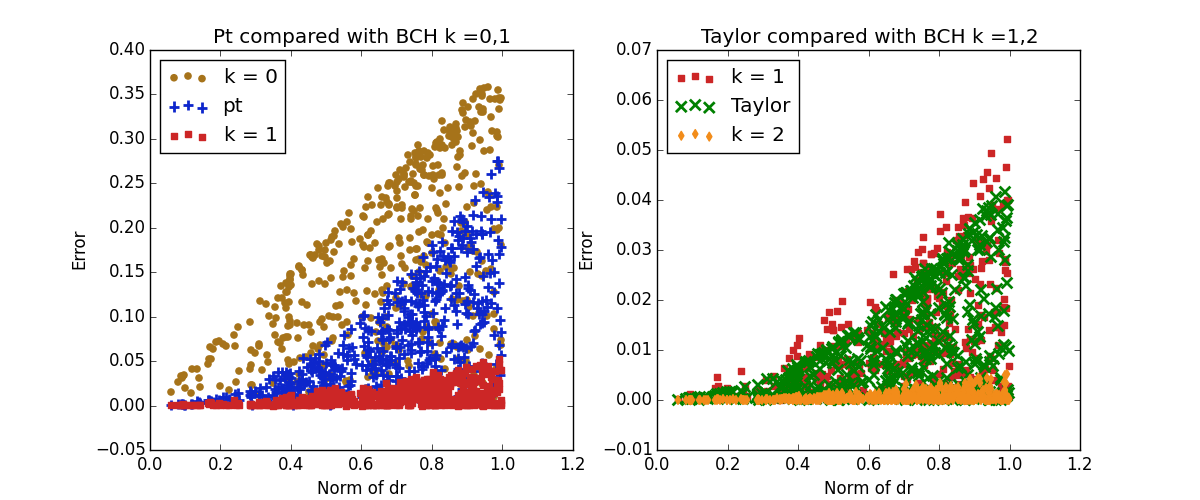
\includegraphics[scale=0.6]{figures/se2_pt_taylor.png}
	\caption{comparisons between Parallel Transport method and Taylor method. TODO}
	\label{fig:se2_pt_taylor}
\end{figure}


\begin{figure}[!ht]
	\hspace{-2cm}
	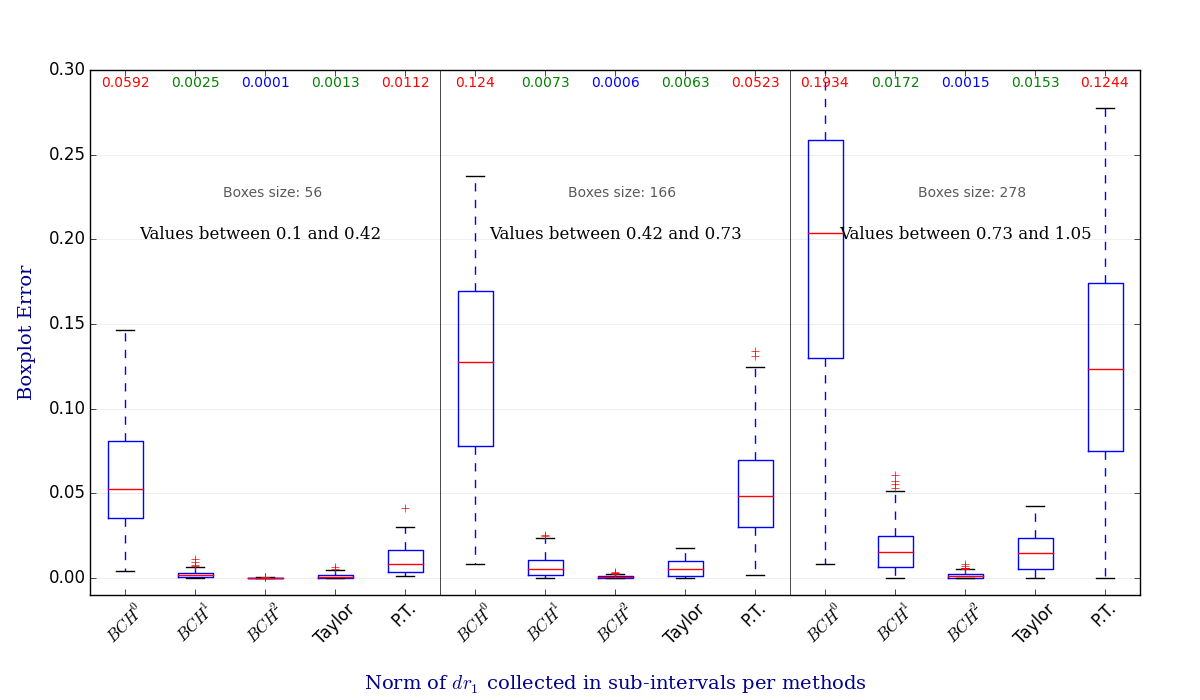
\includegraphics[scale=0.75]{figures/se2_boxplot.png}
	\caption{comparisons between all the methods. TODO}
	\label{fig:se2_boxplot}
\end{figure}


% % % % % % % % % % % % % % % % % % % % % % % % % % % % % % % % % % % % % %
% % % % % % % % % % % % % % % % % % % % % % % % % % % % % % % % % % % % % % 
\subsection{Empirical Evaluations of Computational Time}


% % % % % % % % % % % % % % % % % % % % % % % % % % % % % % % % % % % % % % 
% % % % % % % % % % % % % % % % % % % % % % % % % % % % % % % % % % % % % % 
\section{Log-composition for SVF}
Using a python software, we created synthetic random matrices in $\mathfrak{se}(2)$. We considered the difference between the log composition computed with the closed form \ref{eq:log_composition_se2_closed_form}. 
A sample of $500$ couples $(dr_0,dr_1)$ of elements in $\mathfrak{se}(2)$ are created, 



\begin{figure}[!ht]
	\hspace{-1cm}
	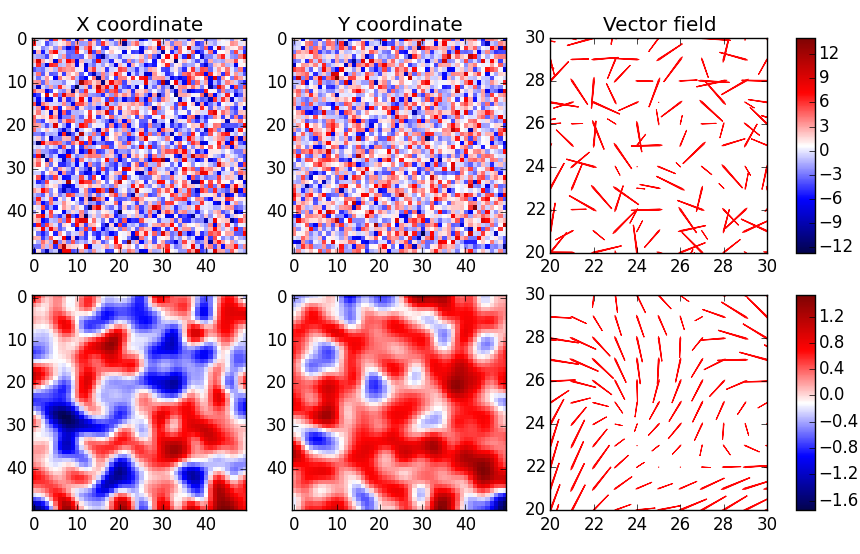
\includegraphics[scale=0.75]{figures/gaussian_smoothing_effect.png}
	\caption{Random generated vector field: }
	\label{fig:svf_gaussian_smoothing_effects}
\end{figure}


% % % % % % % % % % % % % % % % % % % % % % % % % % % % % % % % % % % % % %
% % % % % % % % % % % % % % % % % % % % % % % % % % % % % % % % % % % % % % 
\subsection{Methods}

% % % % % % % % % % % % % % % % % % % % % % % % % % % % % % % % % % % % % %
% % % % % % % % % % % % % % % % % % % % % % % % % % % % % % % % % % % % % % 
\subsection{Results}

% % % % % % % % % % % % % % % % % % % % % % % % % % % % % % % % % % % % % %
% % % % % % % % % % % % % % % % % % % % % % % % % % % % % % % % % % % % % % 
\subsection{Empirical Evaluations of Computational Time}

% % % % % % % % % % % % % % % % % % % % % % % % % % % % % % % % % % % % % %
% % % % % % % % % % % % % % % % % % % % % % % % % % % % % % % % % % % % % % 
% % % % % % % % % % % % % % % % % % % % % % % % % % % % % % % % % % % % % % 
\section{Log-Algorithm for SVF}

% % % % % % % % % % % % % % % % % % % % % % % % % % % % % % % % % % % % % %
% % % % % % % % % % % % % % % % % % % % % % % % % % % % % % % % % % % % % % 
\subsection{Methods}

% % % % % % % % % % % % % % % % % % % % % % % % % % % % % % % % % % % % % %
% % % % % % % % % % % % % % % % % % % % % % % % % % % % % % % % % % % % % % 
\subsection{Results}


% % % % % % % % % % % % % % % % % % % % % % % % % % % % % % % % % % % % % %
% % % % % % % % % % % % % % % % % % % % % % % % % % % % % % % % % % % % % % 
\subsection{Empirical Evaluations of Computational Time}


% % % % % % % % % % % % % % % % % % % % % % % % % % % % % % % % % % % % % %
% % % % % % % % % % % % % % % % % % % % % % % % % % % % % % % % % % % % % %
% % % % % % % % % % % % % % % % % % % % % % % % % % % % % % % % % % % % % % 
\section{Conclusion and Further Research}\label{ch:conclusions}


Considering only the results, this one-year research can be considered much ado about nothing, but...\\
Computational time...!

Starting from the definition of Lie log-group of diffeomorpshisms $(\mathfrak{g} , \oplus)$, to have an algebraic definition of this approximation, we can consider its quotient over the ideal generated by $(\text{ad}_{\mathbf{u}}^{m}, \text{ad}_{\mathbf{u}}^{n})$, which provides the group $(\quotient{\mathfrak{g}}{(\text{ad}_{\mathbf{u}}^{m}, \text{ad}_{\mathbf{u}}^{n})}, \oplus)$. Further investigations in this direction is not prosecuted.
